%\chapter{PyDot library}

\section*{Overview}

This program is writen in python 3.2, and it is written as a project in Visual Studio 2017. In order to execute it from Visual Studio, you need to have installed the following packages:

\begin{itemize}
	\item \textbf{matplolib}
	\item \textbf{PILLOW}
	\item \textbf{PyDot}
	\end{itemize}

 The project consists in three files: One common file that defines the interface (\textit{main.py}), one that handles fortran code (\textit{fortran.py}) and the last one that handles python code (\textit{python.py}). The \textit{fortran.py} code and the \textit{python.py} code use the library PyDot for managing graphs.


\section*{PyDot Library}

This is a library downloaded from \href{https://github.com/erocarrera/pydot}{GitHub}, which author is Ero Carrera. It is a python interface to the GraphViz software, which makes the graphs. More information and installation details are explained in the web page, but in this case you will not need to install it, as it comes with the Software Design source files. 

This file, \textbf{pydot.py}, offers you a few defined classes related to elements of graphs, with which you can build the graph. These are the more relevant:

\begin{itemize}
    \item \textbf{class Graph} Basic element that contains the rest of the classes.
    \item \textbf{class Dot} It is based on the graph, and represents a code writen in dot language
    \item \textbf{class Subgraph} Class representing a subgraph in Graphviz's dot language.
    \item \textbf{class Cluster} Class representing a cluster in Graphviz's dot language.
    \item \textbf{class Node} It creates a node, and you must  add it to a graph, subgraph, cluster or dot class.
    \item \textbf{class Edge} It creates a node between two nodes, and it must be added to the graph, subgraph, cluster or dot class.
\end{itemize}

%\newpage

%
%\chapter{Software Design program}

\section*{Main.py}

The \textit{main.py} file uses the \textbf{matplotlib} library and its widgets, and it interacts with external files, like the configuration file (which saves the previous session parameters), or the list of exclussions \textit{excludes.ini}. This code also defines the GUI itself.

Both files \textit{fortran.py} and \textit{python.py} have a dynamic of searching in the files key words of the code, and building the structure of the program in dictionaries and tuples.

\section*{Fortran.py}
This module is responsible of creating an internal structure by reading the FORTRAN code, and later create the graphs with the \textbf{PyDot} library.

This module uses mainly the following packages: \textbf{re} (Regular Expressions, this is very important because it contains many useful tools for handling text), \textbf{os} (for looking for files) and \textbf{tkinter} (Windows that asks for specific files of directories).

In \textit{fortran.py}, first searches the $USE$ statements from the main file, passing through all files and building a tuple of the structure. This action is carried out mainly by the function \textit{\_\_get\_project\_dependencies} and \textit{\_\_get\_filedependencies} inside the \textit{fortran.py} code.
Later, it searches for the code that defines the types, and it builds again the structure of the types tree.
 For more details, there are comments in the code itself.

\section*{Python.py}
This module is responsible of managing the PYTHON code by reading the code files and creating an internal structure. Later, it uses the \textbf{PyDot} library for generating the graphs.

After the main file is chosen , the program knows that the file is a python code. The main difference with \textit{fortran.py} is that it searches libraries in the python directory.

As \textit{fortran.py}, it uses packages like \textbf{re} and \textbf{os}

\section*{Example of using the PyDot library}

The following is a simple python code that imports the PyDot library. It consists of a graph with three nodes connected, two of which are in a subgraph:

\begin{lstlisting}
from pydot import *

if __name__ == '__main__':


grafico= Dot(graph_name="Prueba",graph_type="digraph")


main_node=Node(name="Nodo1", shape="Mrecord", label="Nodo principal")
sec_node=Node(name="Nodo2", shape="record", label="Nodo secundario")
ter_node=Node(name="Nodo3", shape="",        ) 

label="{N|P}"
sec_node.set_label(label)

main_node.set_label("{Nodoprincipal|"+label+"}")


grafico.add_node(main_node)
grafico.add_node(sec_node)
grafico.add_node(ter_node)

edge=Edge(main_node,sec_node)
edge2=Edge(main_node,ter_node)

grafico.add_edge(edge)
grafico.add_edge(edge2)


zona=Cluster("zona1",label = "Zona 1")

zona.add_node(main_node)
zona.add_node(sec_node)

grafico.add_subgraph(zona)


grafico.write_pdf('prueba.pdf')
\end{lstlisting}
%\vspace{0.1cm}
\begin{center}
\textit{Example code that uses the PyDot library}
\end{center}
\vspace{3cm}
The following is the result of running the previous code (prueba.pdf):

\begin{figure}[H]
    \begin{center}
        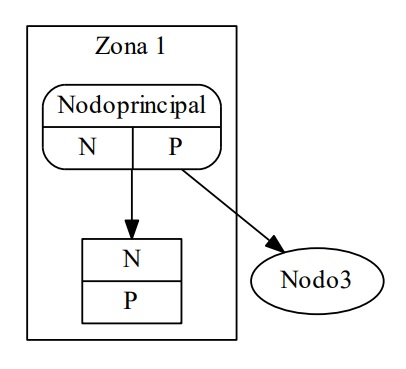
\includegraphics[width=0.4\linewidth]{\home/images/prueba.jpg}
    \end{center}
\end{figure}



